\documentclass[12]{article}
\usepackage{graphicx}
\usepackage{color}
\usepackage{algorithmic}
\begin{document}

\title{\textbf{
\includegraphics[scale=0.5]{42.png}
\textcolor{red}{Universitatea din Craiova \\Facultatea de Automatic\u{a},Calculatoare \c{s}i Electronic\u{a}}}}
\date{\textbf{03 June 2018}}
\maketitle
\begin{center}

\includegraphics[scale=2]{word.jpg}
\end{center}
\textbf{Project : Algorithm Design} \\
\textbf{Title : Crypting and Decrypting of a message}\\
\textbf{Teachers : B\u{a}dic\u{a} Costin \& Ionu\c{t} Murare\c{t}u \& Becheru Alex}\\
\textbf{Student : Laz\u{a}r Leonard Ruben } \\
\textbf{Section : Calculatoare Rom\^{a}n\u{a}\\ Year I\\ Group : 1.2B}
\newpage
\tableofcontents

\newpage
\section{Problem Statement}

\textcolor{white}{}
\subsection{Title}
         \textcolor{blue}    {Crypting and Decrypting of a message}

\subsection{Description}
\textcolor{white}{} 

My project refers to an application that will contain an algorithm for encrypting the relevant characters appear in words with a count that represents a prime number, and an algorithm that will decrypt the encrypted messages in the same manner as the above.  Any string that will appear in a nonprim number is irelevant and ignored by the decrypt function and will be generated randomly to the crypt function.

Dynamic allocation is the automatic allocation of memory in C/C++, Unlike declarations, which load data onto the programs data segment, dynamic allocation creates new usable space on the programs STACK (an area of RAM specifically allocated to that program).For this reason the matrix was dynamically allocated.








\newpage
\section{Pseudocode}


\subsection{prime no} 
\begin{algorithmic}[1] 
\STATE $START$
\STATE $INT \ i,number$ 
\IF{$( number == 0 || number == 1 )$} 
\STATE $not\ a\ prime\ number\ > \ END$
\ENDIF
\FOR{$(i=2$ TO number/2+1} 
    \IF{$(number \% i == 0)$}
    \STATE $not\ a \ prime\ number\ >\ END$
\ENDIF
\ENDFOR

\STATE $ \ prime\ number\ >\ END$


\end{algorithmic} 




\subsection{generate letter} 
\begin{algorithmic}[1] 
\STATE $START$ 
\STATE $int \ pick , var$ 
\STATE $pick = rand() \% 2 $ 
\IF{$(pick == 0)$} 
\STATE $var = rand() \% 26$ 
\STATE $var = var \ + 97$ 
\STATE $*letter = var$  
\ELSE 
\STATE  $var = rand() \% 26$ 
\STATE  $var = var + 65$ 
\STATE  $*letter = var$ 
\ENDIF  
\STATE $END$
\end{algorithmic}

\subsection{generate prime} 

\begin{algorithmic}[1] 
\STATE $START$ 
\STATE $ INT \ i, pick$ 
\STATE $ INT \ stock[6] = {2,3,5,7,11,13} $ 
\STATE $ pick = rand() \% 6 $  
\STATE $*n = stock[pick]$ 
\STATE $END$
\end{algorithmic} 




\subsection{generate non prime} 

\begin{algorithmic}[1] 
\STATE $START$  
\STATE $INT \ pick=2 $ 
\WHILE {$( prime_no( pick ) )$} 
    \STATE $pick = rand()\%14$ 
\ENDWHILE 
\STATE $*n = pick$ 
\STATE $END$
\end{algorithmic} 


\subsection{generate print array} 
\begin{algorithmic}[1] 
\STATE $START$
\STATE $INT \ i$ 
\FOR{$(i=0 \ TO \ array.size)$} 
\STATE $print("\%c", array.text[i])$   
\ENDFOR
\STATE $END$
\end{algorithmic} 


\subsection{Message Decrypt} 
\begin{algorithmic}[1] 
\STATE $START$
\STATE $char \ letter = '+'$
\STATE $char \ last_letter = '*'$
\STATE $INT \ i, apparitions = 1 $  
\STATE $d \_array.size = 0$
\STATE $d \_array.text = (char *) malloc(d\_array.size * sizeof(char))$ 
\FOR{$(i=0 \ TO \ array.size + 2)$} 
    \IF{$( letter != last \_letter )$} 
        \IF{$( prime \_no( apparitions ) )$} 
                \STATE $d \_array.size++$
                \STATE $d \_array.text = (char *)realloc( d \_array.text, d \_array.size * sizeof(char) )$
                \STATE $d \_array.text[d \_array.size - 1] = last \_letter$ 
        \ENDIF 
    \STATE $apparitions = 1$
    \STATE $last_letter = letter$
    \STATE $letter = array.text[i]$ 
    \ENDIF 
\ENDFOR 
\STATE$END$
\end{algorithmic}  


\subsection{Message Crypt} 
\begin{algorithmic}[1] 
\STATE $START$
\STATE $char letter$ 
\STATE $INT\ i,\ j = 0 , \ letter \_num, \ flag  $ 
\FOR{$(i=0 \ TO \_array.size$} 
    \STATE $flag = rand() \% 2$ 
        \WHILE{$(flag)$} 
            \STATE $generate\_letter( \&letter )$
            \STATE $generate\_non\_prime( \&letter\_num )$
            \STATE $c_array.size += letter_num$
            \STATE$c\_array.text = (char *) realloc( c \_array.text, c \_array.size)$
                \FOR{$(j \ TO \ c \_array.size)$} 
                     \STATE $c_array.text[j] = letter$ 
                \ENDFOR 
            \STATE $flag = rand() \% 2$ 
        \ENDWHILE  
    \STATE $generate_prime( \&letter\_num )$
    \STATE $c\_array.size += letter\_num$
    \STATE $c \_array.text = (char *) realloc( c\_array.text, c\_array.size)$ 
        \FOR{$(j \ TO \ c \_array.size)$}  
            \STATE$c_array.text[j] = array.text[i]$ 
        \ENDFOR 
\ENDFOR 
\STATE$END$
\end{algorithmic}  


\newpage
\section{Application Design}
\subsection{Main}
\textbf{} 



This module contains only the main function. The user is required to introduce an input from the keyboard. First of all,we will need to count if a string represents a prime number or not,for this issue we will implement prime\_no function that will check if a number is prime, we will implement generate\_letter function that will generate a random letter ,we will implement generate\_prime function that will generate a non prime number from 1 to 14 because otherwise the output couldn't have been human readable , we will implement generate\_prime function that will generate a prime number from 2 to 13 and we will declare an array used to store the first 6 prime numbers , only those were used to ease the readability of crypted messages output. For this program I used the crypt and the decrypt function. For the encryption function I used the parameter c\_array.size where I will stock the message that will be encrypted,with the help of the variables letter and last\_letter I will store the current letter and the precedent letter,also I count the number of apparitions of a letter with the variable apparitions,also I used a flag variable like this : when (flag == 1) then there will be a non prime array of letters,and in the end I used the structure variable c\_array witch will store the encrypted message. For the decryption function  I used the parameter d\_array.size where I will stock the message that will be decrypted,with the help of the variables letter and last\_letter I will store the current letter and the precedent letter,also I count the number of apparitions of a letter with the variable apparitions,and in the end I used the structure variable d\_array witch will store the decrypted message.
There is a chance that in between every good sequence of letters a bad non-readable sequence will be added as it was specified in the problem requirements (a prime number of letters sequence), this chance is determined by the function rand() and the good and bad sequences will be generated by the following functions : generate\_prime() , generate\_non\_prime() , generate\_letter().
The main function contains only functions calls.  
















\subsection{Input Data}
\textcolor{white}{} 
 
 
 In my implementation I decided to require the used to introduce from the keyboard an already encrypted message following the problem requirements ( only prime rows of the same letter will be counted as a good set of data and decrypted with that specific letter ) This message will be decrypted and crypted again in order to show that both of the functions work as intended . 










\subsection{Output Data}
\textcolor{white}{}  



The output data of my implementation will be shown on the run screen to ease its readability for the user. The output will be represented by the decrypted message initially and then by the respective crypted message as I already specified in the input subsection.












\subsection{Functions}
\textcolor{white}{}

The functions used in the program are presented in \textbf{Section 2},where is presented and pseudocode.





\section{Source Code}

\textcolor{white}{}


My project is called ``Crypting and Decrypting of a message`` . The source code is created in  programming language standard C99,that is compiled in one  compiler. The  compiler is in \textcolor{blue}{GNU GCC Compiler} with help program Code Blocks 16.01 

\newpage
\section{Experiments and results}
\textcolor{white}{}
\subsection{GNU GCC Compiler}
For the GCC compiler, will present a case. The method I used, running the program in the next subsection. 

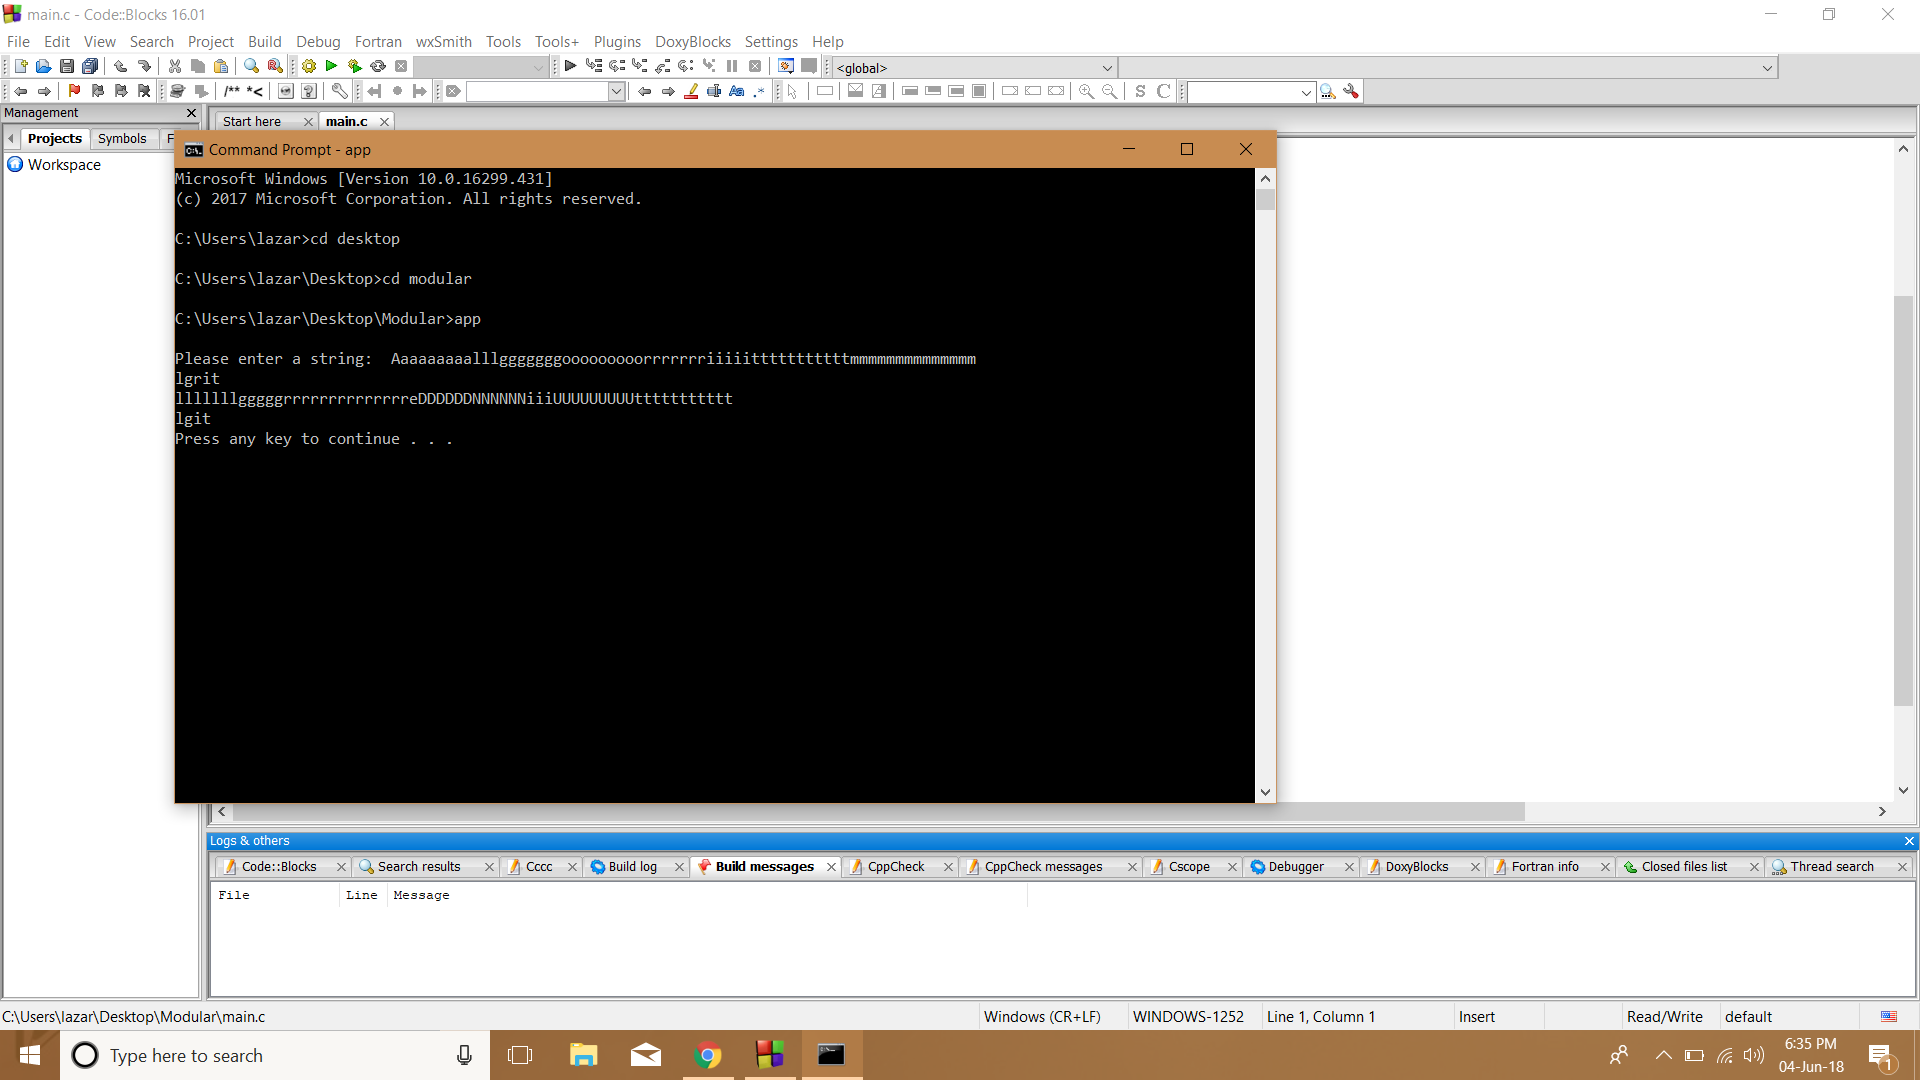
\includegraphics[scale=0.3]{pro.jpg} 



\newpage
\section{Conclusion}
\textbf{} 

A problem about crypting and decrypting a text is an interesting approach over concepts used in real life in domains such as data bases or even banking , I believe that understanding this concept even at a base level  as it was implemented in this module is very important in order to be able to develop and work in a more complex work environment that requires data security that can only be obtained through encryption.



\newpage
\section{References}

\textbf{Book}:

Name : Totul despre C si C++ 

Year of publication  :2005

Publishing :Teora

Author :Dr. Kris Jamsa Lars Klander\\
\textbf{Web references}:

$1.http://www.geeksforgeeks.org$

$2. https://www.sharelatex.com/learn/Main_Page$\\
\textbf{Article}:

$1. https://en.wikipedia.org/wiki/Encryption$


\end{document}